\subsubsection{Achromatic polarization rotation around compact objects (EHT intercept test)}
\label{sec:eht-intercept}
%-----------------------------------------------------------------------------

Beyond the cosmic birefringence prediction (Theorem~\ref{thm:birefringence}), TFPT implies a local, achromatic polarization rotation
in the presence of a nonzero $E\cdot B$ environment (see the companion note \cite{bhAchromaticRotationNote2025}). EHT-style polarimetry
provides the relevant data products for such an intercept test \cite{ehtm87pol2021}. A simple dyonic toy model yields
\begin{equation}
\beta_{\mathrm{BH}}(r_{\mathrm{em}})
:= \frac{1}{256\pi^4}\,\frac{Q^{\mathrm{eff}}_e Q^{\mathrm{eff}}_m}{r_{\mathrm{em}}^2},
\end{equation}
where $r_{\mathrm{em}}$ is the emission radius and $Q^{\mathrm{eff}}_{e,m}$ denote effective electromagnetic charges sourcing $E\cdot B$ along the line of sight. A toy derivation of the $1/r^2$ scaling is given in Appendix~\ref{app:bh-dyonic}.

\textbf{Observation strategy (EHT style).}
At each image pixel $x$, fit the electric vector position angle (EVPA) across frequencies by
\begin{equation}
\chi(\lambda^2,x)=\chi_0(x)+\mathrm{RM}(x)\lambda^2,
\end{equation}
and interpret $\chi_0(x)$ as the achromatic intercept map. A nonzero intercept pattern correlated
with emission radius and polarization structure provides a direct falsifiable test.

\begin{tcolorbox}[colback=gray!5, colframe=gray!60, breakable,
title={\textbf{EHT Intercept Map Procedure (achromatic intercept $\chi_0$)}}, fonttitle=\bfseries\small]
\begin{itemize}[leftmargin=1.5em, topsep=2pt, itemsep=2pt]
    \item For each pixel $x$, fit $\chi(\lambda^2,x)$ across bands to $\chi_0(x)+\mathrm{RM}(x)\lambda^2$.
    \item Treat $\chi_0(x)$ as the \emph{achromatic} intercept map (TFPT observable).
    \item Treat $\mathrm{RM}(x)$ as a Faraday-rotation nuisance map (astrophysical foreground / plasma).
    \item The primary null test is $\chi_0(x)=0$ (up to instrumental calibration); a robust nonzero pattern is the signal channel.
    \item Achromaticity check: $\chi_0(x)$ is stable under band splits; residual frequency dependence belongs in $\mathrm{RM}(x)$.
    \item Control sources: apply the same fit to calibrators or off-source regions; expect $\chi_0(x)\approx 0$.
    \item Sign/handedness check: a parity flip or Stokes $Q/U$ sign inversion should flip $\chi_0$; failure indicates systematics.
\end{itemize}
\end{tcolorbox}

\begin{figure}[H]
\centering
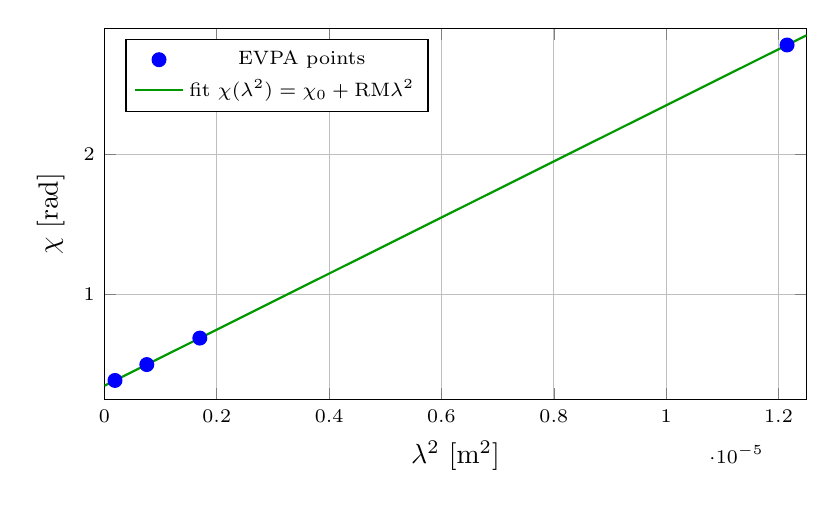
\begin{tikzpicture}
\begin{axis}[
    width=10.5cm, height=6.3cm,
    xlabel={$\lambda^2$ [m$^2$]},
    ylabel={$\chi$ [rad]},
    xmin=0, xmax=1.25e-5,
    ymin=0.25, ymax=2.9,
    grid=major,
    scaled x ticks=true,
    tick label style={font=\scriptsize},
    legend style={font=\scriptsize},
    legend pos=north west
]
    \addplot[only marks, mark=*, mark size=2.5pt, blue] coordinates {
        (1.215190885258e-05,2.780382)
        (1.698970092130e-06,0.689794)
        (7.550978187245e-07,0.501020)
        (1.887744546811e-07,0.387755)
    };
    \addlegendentry{EVPA points}

    \addplot[thick, green!60!black] coordinates {(0,0.35) (1.25e-5,2.85)};
    \addlegendentry{fit $\chi(\lambda^2)=\chi_0+\mathrm{RM}\lambda^2$}

    \node[anchor=south west, font=\scriptsize] at (axis cs:0.25e-6,2.55) {$\chi_0\neq 0$};
\end{axis}
\end{tikzpicture}
\caption{Schematic EVPA fit: an achromatic intercept $\chi_0$ plus a Faraday term $\mathrm{RM}\lambda^2$. The intercept map extracted from multi-frequency imaging is the primary TFPT observable.}
\label{fig:evpa_intercept}
\end{figure}

%-----------------------------------------------------------------------------
\subsection{Gravitational Coupling from Invariants}
%-----------------------------------------------------------------------------

\begin{corollary}{Gravitational Coupling Consistency}{kappa}
The gravitational coupling $\kappa^2 = 8\pi G$ (with dimension $[\text{energy}]^{-2}$) 
is constrained by consistency with the dimensionless ratio:
\begin{equation}
    \xi \equiv \frac{\cthree}{\phiz}
\end{equation}

\textbf{Dimensional analysis:} Both $\cthree$ and $\phiz$ are dimensionless. The 
physical gravitational coupling $G$ enters when restoring dimensions:
\begin{equation}
    \kappa^2 = 8\pi G = \frac{1}{\Mpl^2}
\end{equation}
The TFPT claim is that the \emph{ratio} $\cthree/\phiz$ is fixed by topology, 
not that $G$ is derived from dimensionless constants alone.

\textbf{Tree-level value:} With $\phitree = 1/(6\pi)$ and $\cthree = 1/(8\pi)$:
\begin{equation}
    \xi_{\text{tree}} = \frac{1/(8\pi)}{1/(6\pi)} = \frac{6\pi}{8\pi} = \frac{3}{4}
\end{equation}

\textbf{With backreaction:} Using $\phiz \approx 0.05317$:
\begin{equation}
    \xi = \frac{0.03979}{0.05317} \approx 0.7483
\end{equation}
This is a shift of $-0.22\%$ from the tree-level value.

\textbf{Physical interpretation:} The ratio $\xi$ determines the relative strength 
of axion-mediated and gravitational interactions. It is \emph{not} a derivation of 
Newton's constant $G$, which remains an input (via $M_{\text{Pl}}$).
\end{corollary}

%=============================================================================
\section{Observable Predictions}
%=============================================================================

%-----------------------------------------------------------------------------
\subsection{Axion--Photon Coupling}
%-----------------------------------------------------------------------------

\begin{corollary}{Axion--Photon Coupling}{gagg}
The CFE fixes the axion--photon vertex uniquely:
\begin{equation}
    \boxed{\gagg = -4\cthree = -\frac{1}{2\pi} \approx -0.1592}
\end{equation}
This determines cosmic birefringence without free parameters.
\end{corollary}

%-----------------------------------------------------------------------------
\subsection{Cosmic Birefringence}
%-----------------------------------------------------------------------------

\begin{definition}{Topological Excursion Quantization}{topoexcursion}
The topological axion excursion is quantized in discrete sector changes:
\begin{equation}
    \Delta a_{\text{top}} = n\,\phiz, \qquad n\in\mathbb{Z},
\end{equation}
with $n=1$ the minimal nontrivial class. The corresponding birefringence is
$\beta = \Delta a_{\text{top}}/(4\pi) = n\,\phiz/(4\pi)$.
\end{definition}

\begin{theorem}{Cosmic Birefringence Prediction}{birefringence}
A homogeneous topological axion field $a_{\text{top}}(\eta)$ rotates the polarization plane of light by:
\begin{equation}
    \frac{d\beta}{d\eta} = 2\cthree\frac{da_{\text{top}}}{d\eta} 
    \quad\Rightarrow\quad 
    \beta = \frac{\Delta a_{\text{top}}}{4\pi}
\end{equation}
Using the coupling convention $\gagg=-4\cthree$ (Corollary~\ref{cor:gagg}) and the sign convention for $\beta$ stated below, the transport law is equivalently
$\frac{d\beta}{d\eta} = -\frac{1}{2}\gagg\,\frac{da_{\text{top}}}{d\eta} = 2\cthree\,\frac{da_{\text{top}}}{d\eta}$.
With the minimal nontrivial sector $n=1$ (Definition~\ref{def:topoexcursion}):
\begin{equation}
    \boxed{\beta_{\text{th}} = \frac{\phiz}{4\pi} = 0.0042312895\ldots~\text{rad} = 0.2424^\circ}
\end{equation}
\end{theorem}

\begin{tcolorbox}[colback=yellow!3, colframe=yellow!60!black,
    title={\textbf{Sign conventions for $\beta$}}, fonttitle=\bfseries\small]
\textbf{Sign:} $\beta>0$ corresponds to a counter-clockwise rotation of linear polarization
when looking toward the source (Planck/ACT convention).
\textbf{Units:} $\beta$ is quoted in radians unless a degree symbol is shown explicitly.
\end{tcolorbox}

\subsubsection{Dynamical Completion of the Excursion}
\label{sec:deltaa}

\begin{tcolorbox}[colback=red!3, colframe=red!50!black, 
    title={\textbf{One Minimal Dynamical Realization: Late-Time Shifted Axion Attractor}}, fonttitle=\bfseries\small]
\textbf{Goal:} Provide one minimal dynamical realization compatible with the topological quantization (Definition~\ref{def:topoexcursion}).

\textbf{Shifted periodic potential:} The smallest periodic completion that enforces the geometric shift is
\begin{equation}
    V(a_{\text{top}},t)=\Lambda^4\Bigl[1-\cos\bigl(a_{\text{top}}-\phiz\,s(t)\bigr)\Bigr],
    \label{eq:shifted-axion-potential}
\end{equation}
where $s(t)$ transitions from $0$ to $1$ at late times (e.g.\ when a TFPT block becomes dynamically relevant).
Then the instantaneous minimum shifts from $a=0$ (early) to $a=\phiz$ (late).

\textbf{Attractor consequence (conditional):} If a late-time transition occurs after recombination and the background mode relaxes toward the new minimum,
\begin{equation}
    \Delta a_{\text{top}} = a_{\text{top}}(t_0)-a_{\text{top}}(t_{\mathrm{rec}}) \simeq \phiz \quad (n=1)
    \quad\Rightarrow\quad
    \beta \simeq \frac{\phiz}{4\pi},
\end{equation}
recovering the TFPT birefringence prediction as an attractor rather than a bare assumption.

\textbf{Timing without continuous tuning (one realization):} The effective mass is $m_{\mathrm{eff}}\sim \Lambda^2/f_a$.
Requiring $m_{\mathrm{eff}}\sim H_0$ delays the roll to very late times (robustly after recombination). With $f_a\sim 10^{11}$~GeV this corresponds to
$\Lambda\sim \sqrt{H_0 f_a}\sim 10^{-6}$~eV (order-of-magnitude).

\textbf{Discrete realization via a TFPT block (optional):} One may treat $\Lambda$ itself as the scale of an additional ultra-light TFPT block,
generated by the same universal suppression $\zeta_B \sim (\pi\cthree)\exp(-\beta_B\pi\cthree)\exp(-k_B/\cthree)$ with $k_B=\frac{3}{2}I_1(B)$.
A minimal rational charge set $\{1,2/3,2/3\}$ gives $I_1=1+2\cdot(4/9)=17/9$ and $k=17/6$, yielding $\Lambda$ naturally in the $\mu$eV range for late cascade levels,
and hence $m_{\mathrm{eff}}\sim 10^{-32}$~eV (cosmologically late roll) without introducing a continuous tuning knob.

\textbf{New test:} If the field is still evolving today, birefringence becomes redshift-dependent:
\begin{equation}
    \beta(z)=\frac{a(t_0)-a(t(z))}{4\pi}.
\end{equation}
This can be constrained by birefringence tomography using CMB and polarized sources across redshift.
\end{tcolorbox}

\begin{tcolorbox}[colback=orange!5, colframe=orange!60!black, 
    title={\textbf{Sign Convention for Birefringence}}, fonttitle=\bfseries\small]
\textbf{Definition:} $\beta > 0$ corresponds to a counter-clockwise rotation of the 
polarization plane when looking along the photon propagation direction (IAU convention).

\textbf{Relation to data pipelines:}
\begin{itemize}[leftmargin=1.5em, topsep=2pt, itemsep=1pt]
    \item Planck PR4: Reports $\beta$ in this convention. Our $\beta_{\text{th}} = +0.2424^\circ$ 
        is directly comparable.
    \item ACT DR6: Uses same sign convention; recent result $\beta = 0.215^\circ \pm 0.074^\circ$ 
        is consistent with TFPT at $0.4\sigma$.
    \item Some analyses use $\beta \equiv -\beta_{\text{obs}}$; we do \emph{not} adopt this.
\end{itemize}

\textbf{Dominant systematic:} Absolute polarization angle calibration (via Crab nebula or 
EB-nulling on Galactic dust). Current calibration uncertainty $\sim 0.1^\circ$ is comparable 
to statistical errors.
\end{tcolorbox}

\begin{table}[H]
\centering
\begin{tabular}{@{}lccccc@{}}
\toprule
\textbf{Planck PR4 Case} & $\beta_{\text{obs}}$ [$^\circ$] & $1\sigma$ [$^\circ$] & 
    $\beta_{\text{th}}$ [$^\circ$] & $|\Delta|/\sigma$\\
\midrule
Full-sky (raw EB) & 0.30 & 0.11 & 0.2424 & 0.52\\
Foreground-corrected & 0.36 & 0.11 & 0.2424 & 1.07\\
COMMANDER template & 0.16 & 0.05 & 0.2424 & 1.65\\
\bottomrule
\end{tabular}
\caption{Cosmic birefringence: TFPT prediction vs.\ Planck PR4 observations.}
\label{tab:birefringence}
\end{table}

\begin{figure}[H]
\centering
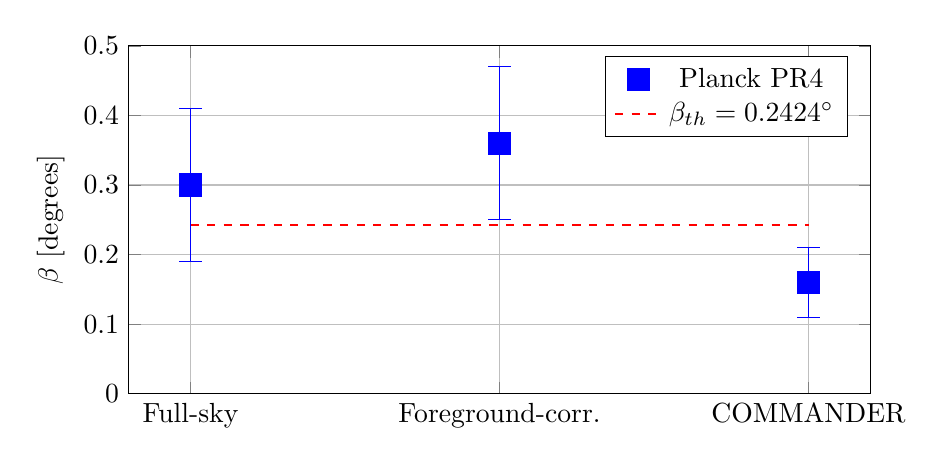
\begin{tikzpicture}
\begin{axis}[
    width=11cm, height=6cm,
    ylabel={$\beta$ [degrees]},
    symbolic x coords={Full-sky, Foreground-corr., COMMANDER},
    xtick=data,
    ymin=0, ymax=0.5,
    ytick={0, 0.1, 0.2, 0.3, 0.4, 0.5},
    grid=major,
    legend pos=north east,
]
    % Observations with error bars
    \addplot[
        only marks,
        mark=square*,
        mark size=4pt,
        blue,
        error bars/.cd,
        y dir=both, y explicit
    ] coordinates {(Full-sky,0.30) +- (0,0.11) (Foreground-corr.,0.36) +- (0,0.11) (COMMANDER,0.16) +- (0,0.05)};
    \addlegendentry{Planck PR4}
    
    % Theory line
    \addplot[thick, red, dashed, domain=0:3] coordinates {(Full-sky,0.2424) (Foreground-corr.,0.2424) (COMMANDER,0.2424)};
    \addlegendentry{$\beta_{\text{th}} = 0.2424^\circ$}
\end{axis}
\end{tikzpicture}
\caption{Cosmic birefringence: TFPT prediction compared with Planck PR4 
measurements. Theory is within 0.5--1.7$\sigma$ of all observations.}
\label{fig:birefringence}
\end{figure}

\begin{figure}[H]
\centering
\begin{tikzpicture}
\begin{groupplot}[
    group style={group size=2 by 1, horizontal sep=1.2cm},
    width=0.48\linewidth,
    height=0.42\linewidth,
    grid=major,
    legend style={font=\scriptsize},
]
\nextgroupplot[
    title={Low-$z$ tomography},
    xlabel={redshift $z$},
    ylabel={$\beta(z)$ [rad]},
    xmin=0, xmax=10,
    xtick={0,1,2,5,10},
]
\addplot+[only marks, mark=o, error bars/.cd, y dir=both, y explicit] coordinates {
    (0.425,0.03490658503988659) +- (0,0.03490658503988659)
    (0.428,0.017453292519943295) +- (0,0.15707963267948966)
    (0.5524,0.22689280275926285) +- (0,0.3490658503988659)
    (0.6897,-0.13962634015954636) +- (0,0.20943951023931956)
    (0.8108,0.0) +- (0,0.17453292519943295)
};
\addlegendentry{low-$z$ (tomography)}
\addplot[domain=0:10, samples=200, thick] {0.004231289511395415*0.5*(1+tanh(min(20,(x-0.0)/0.02)))};
\addlegendentry{best-fit step}
\addplot[domain=0:10, samples=200, thick] {0.004231289511395415*(1-(1+x)^(-10))};
\addlegendentry{best-fit drift}

\nextgroupplot[
    title={CMB anchor},
    xlabel={redshift $z$},
    xmin=900, xmax=1200,
    xtick={900,1000,1100,1200},
    ymin=0, ymax=0.01,
]
\addplot+[only marks, mark=square*, error bars/.cd, y dir=both, y explicit] coordinates {
    (1100,0.0037524578917878084) +- (0,0.0012915436464758037)
    (1100,0.006108652381980153) +- (0,0.0024434609527920616)
    (1100,0.005235987755982988) +- (0,0.0019198621771937625)
    (1100,0.005969026041820607) +- (0,0.0016231562043547264)
};
\addlegendentry{CMB (offset checks)}
\addplot[domain=900:1200, samples=120, thick] {0.004231289511395415*0.5*(1+tanh(min(20,(x-0.0)/0.02)))};
\addlegendentry{best-fit step}
\addplot[domain=900:1200, samples=120, thick] {0.004231289511395415*(1-(1+x)^(-10))};
\addlegendentry{best-fit drift}
\end{groupplot}
\end{tikzpicture}
\caption{Cosmic birefringence tomography. Left: low-$z$. Right: CMB anchor.}
\label{fig:beta-tomography}
\end{figure}

%-----------------------------------------------------------------------------
\subsection{Two-Loop RG Fingerprints}
%-----------------------------------------------------------------------------

\begin{corollary}{RG Fingerprints}{RGfingerprints}
The TFPT invariants leave signatures in the RG flow of gauge couplings:
\begin{align}
    \alpha_3(1\,\text{PeV}) &\approx \phiz \quad 
        \text{(two-loop extrapolated: } \num[round-mode=places,round-precision=6]{\TFPTalphaThreePeVNum}, \text{ dev: } -\num[round-mode=places,round-precision=3]{\TFPTalphaThreePeVRelDevPercent}\%\text{)}\\
    \alpha_3(\mu_{\cthree}) &\approx \cthree \quad 
        \text{(crossing at } \mu_{\cthree}\approx \num[round-mode=places,round-precision=3]{\TFPTmuCrosscThreeGeV}\ \text{GeV, dev: } 0.00\%\text{, by construction)}
\end{align}
These values are obtained by two-loop RG running from PDG boundary conditions at $M_Z$ using the declared PyR@TE model (checked by \texttt{two\_loop\_rg\_fingerprints} in the verification suite; not direct measurements at the quoted scales). The crossing scale for $\alpha_3(\mu)=\phiz$ is $\mu\approx \num[round-mode=places,round-precision=0]{\TFPTmuCrossVarphiZeroGeV}$~GeV.
\end{corollary}

\pgfplotstableread[col sep=comma]{
muGeV,log10mu,alphaY,alpha1GUT,alpha2,alpha3,yt,yb,ytau,lambdaH
91.1876,1.9599,0.01016,0.01694,0.03380,0.11790,0.94,0.017,0.01,0.13
114.86,2.0602,0.01019,0.01699,0.03373,0.11432,0.926,0.0167,0.0100,0.125
458.76,2.6616,0.01035,0.01726,0.03332,0.09673,0.855,0.0151,0.0101,0.102
1154.86,3.0625,0.01046,0.01744,0.03305,0.08777,0.817,0.0142,0.0102,0.090
4612.56,3.6639,0.01064,0.01773,0.03264,0.07709,0.767,0.0131,0.0102,0.076
14625.83,4.1651,0.01078,0.01797,0.03232,0.07000,0.732,0.0124,0.0102,0.066
46376.60,4.6663,0.01093,0.01822,0.03199,0.06412,0.701,0.0117,0.0102,0.058
147054.15,5.1675,0.01108,0.01847,0.03167,0.05916,0.674,0.0112,0.0102,0.051
466289.51,5.6687,0.01124,0.01874,0.03136,0.05492,0.649,0.0107,0.0102,0.045
1478543.15,6.1698,0.01141,0.01901,0.03105,0.05125,0.626,0.0102,0.0102,0.040
4688267.27,6.6710,0.01157,0.01929,0.03075,0.04804,0.606,0.0098,0.0102,0.036
14865883.39,7.1722,0.01175,0.01958,0.03046,0.04521,0.587,0.0094,0.0102,0.032
47137775.20,7.6734,0.01192,0.01987,0.03016,0.04270,0.570,0.0091,0.0102,0.029
1.57e17,17.1958,0.01671,0.02785,0.02548,0.02082,0.371,0.0055,0.0091,0.015
3.95e17,17.5967,0.01700,0.02833,0.02531,0.02038,0.366,0.0055,0.0090,0.016
9.95e17,17.9976,0.01729,0.02882,0.02515,0.01996,0.360,0.0054,0.0090,0.016
2.50e18,18.3986,0.01760,0.02934,0.02499,0.01956,0.355,0.0053,0.0089,0.016
6.30e18,18.7995,0.01792,0.02987,0.02483,0.01917,0.350,0.0052,0.0089,0.017
1.59e19,19.2005,0.01825,0.03042,0.02467,0.01880,0.345,0.0051,0.0088,0.017
}\RgTable
\begin{figure}[H]
\centering
\begin{tikzpicture}
\begin{axis}[
    xmode=log,
    width=0.9\linewidth,
    height=0.48\linewidth,
    xlabel={$\mu$ [GeV]},
    ylabel={$\alpha_i(\mu)$},
    title={Two-loop gauge running (PyR@TE3 numeric solve)},
    grid=both,
    legend pos=north east
]
\addplot table[x=muGeV, y=alpha1GUT]{\RgTable};
\addlegendentry{$\alpha_1=(5/3)\alpha_Y$}
\addplot table[x=muGeV, y=alpha2]{\RgTable};
\addlegendentry{$\alpha_2$}
\addplot table[x=muGeV, y=alpha3]{\RgTable};
\addlegendentry{$\alpha_3$}
\addplot[black, dashed] coordinates {(1e6,0.01) (1e6,0.12)};
\addlegendentry{1 PeV}
\addplot[black, dotted] coordinates {(1e2,0.053171952176845526) (1e19,0.053171952176845526)};
\addlegendentry{$\varphi_0$}
\addplot[gray, dotted] coordinates {(1e2,0.039788735772973836) (1e19,0.039788735772973836)};
\addlegendentry{$c_3$}
\end{axis}
\end{tikzpicture}
\caption{Two-loop gauge running (PyR@TE). $\alpha_i(\mu)$ trajectories with TFPT invariant crossings highlighted.}
\label{fig:rg-two-loop-running}
\end{figure}

%=============================================================================
% PART II: STRUCTURAL EXTENSIONS
%=============================================================================
\vspace{1em}
\begin{center}
\rule{0.8\textwidth}{0.5pt}\\[0.5em]
{\Large\bfseries Part II: Structural Extensions}\\[0.3em]
{\small The following sections extend the core CFE framework. They are \\
testable structural postulates that do not affect the $\alpha$, $\beta$, \\
or RG fingerprint predictions established in Part I; for a PRL-style core \\
presentation they can be treated as companion/supplement material.}\\[0.5em]
\rule{0.8\textwidth}{0.5pt}
\end{center}
\vspace{1em}

%=============================================================================
